\chapter{Laser Pieces}
%the sum of the whole is greater than the parts 


The purpose of this system is to produce two lasers which are near resonant with the 5s $^2$S$_{1/2}$ to 5p$^2$P$_{3/2}$ transition in $^{87}$Sr$+$, but which differ in frequency by precisely the hyperfine ground state splitting. 

This is necessary to make the stimulated Raman transitions for our experiment. 

The laser system consists of several components arranged together on a breadboard. 

\begin{figure}
    \centerline{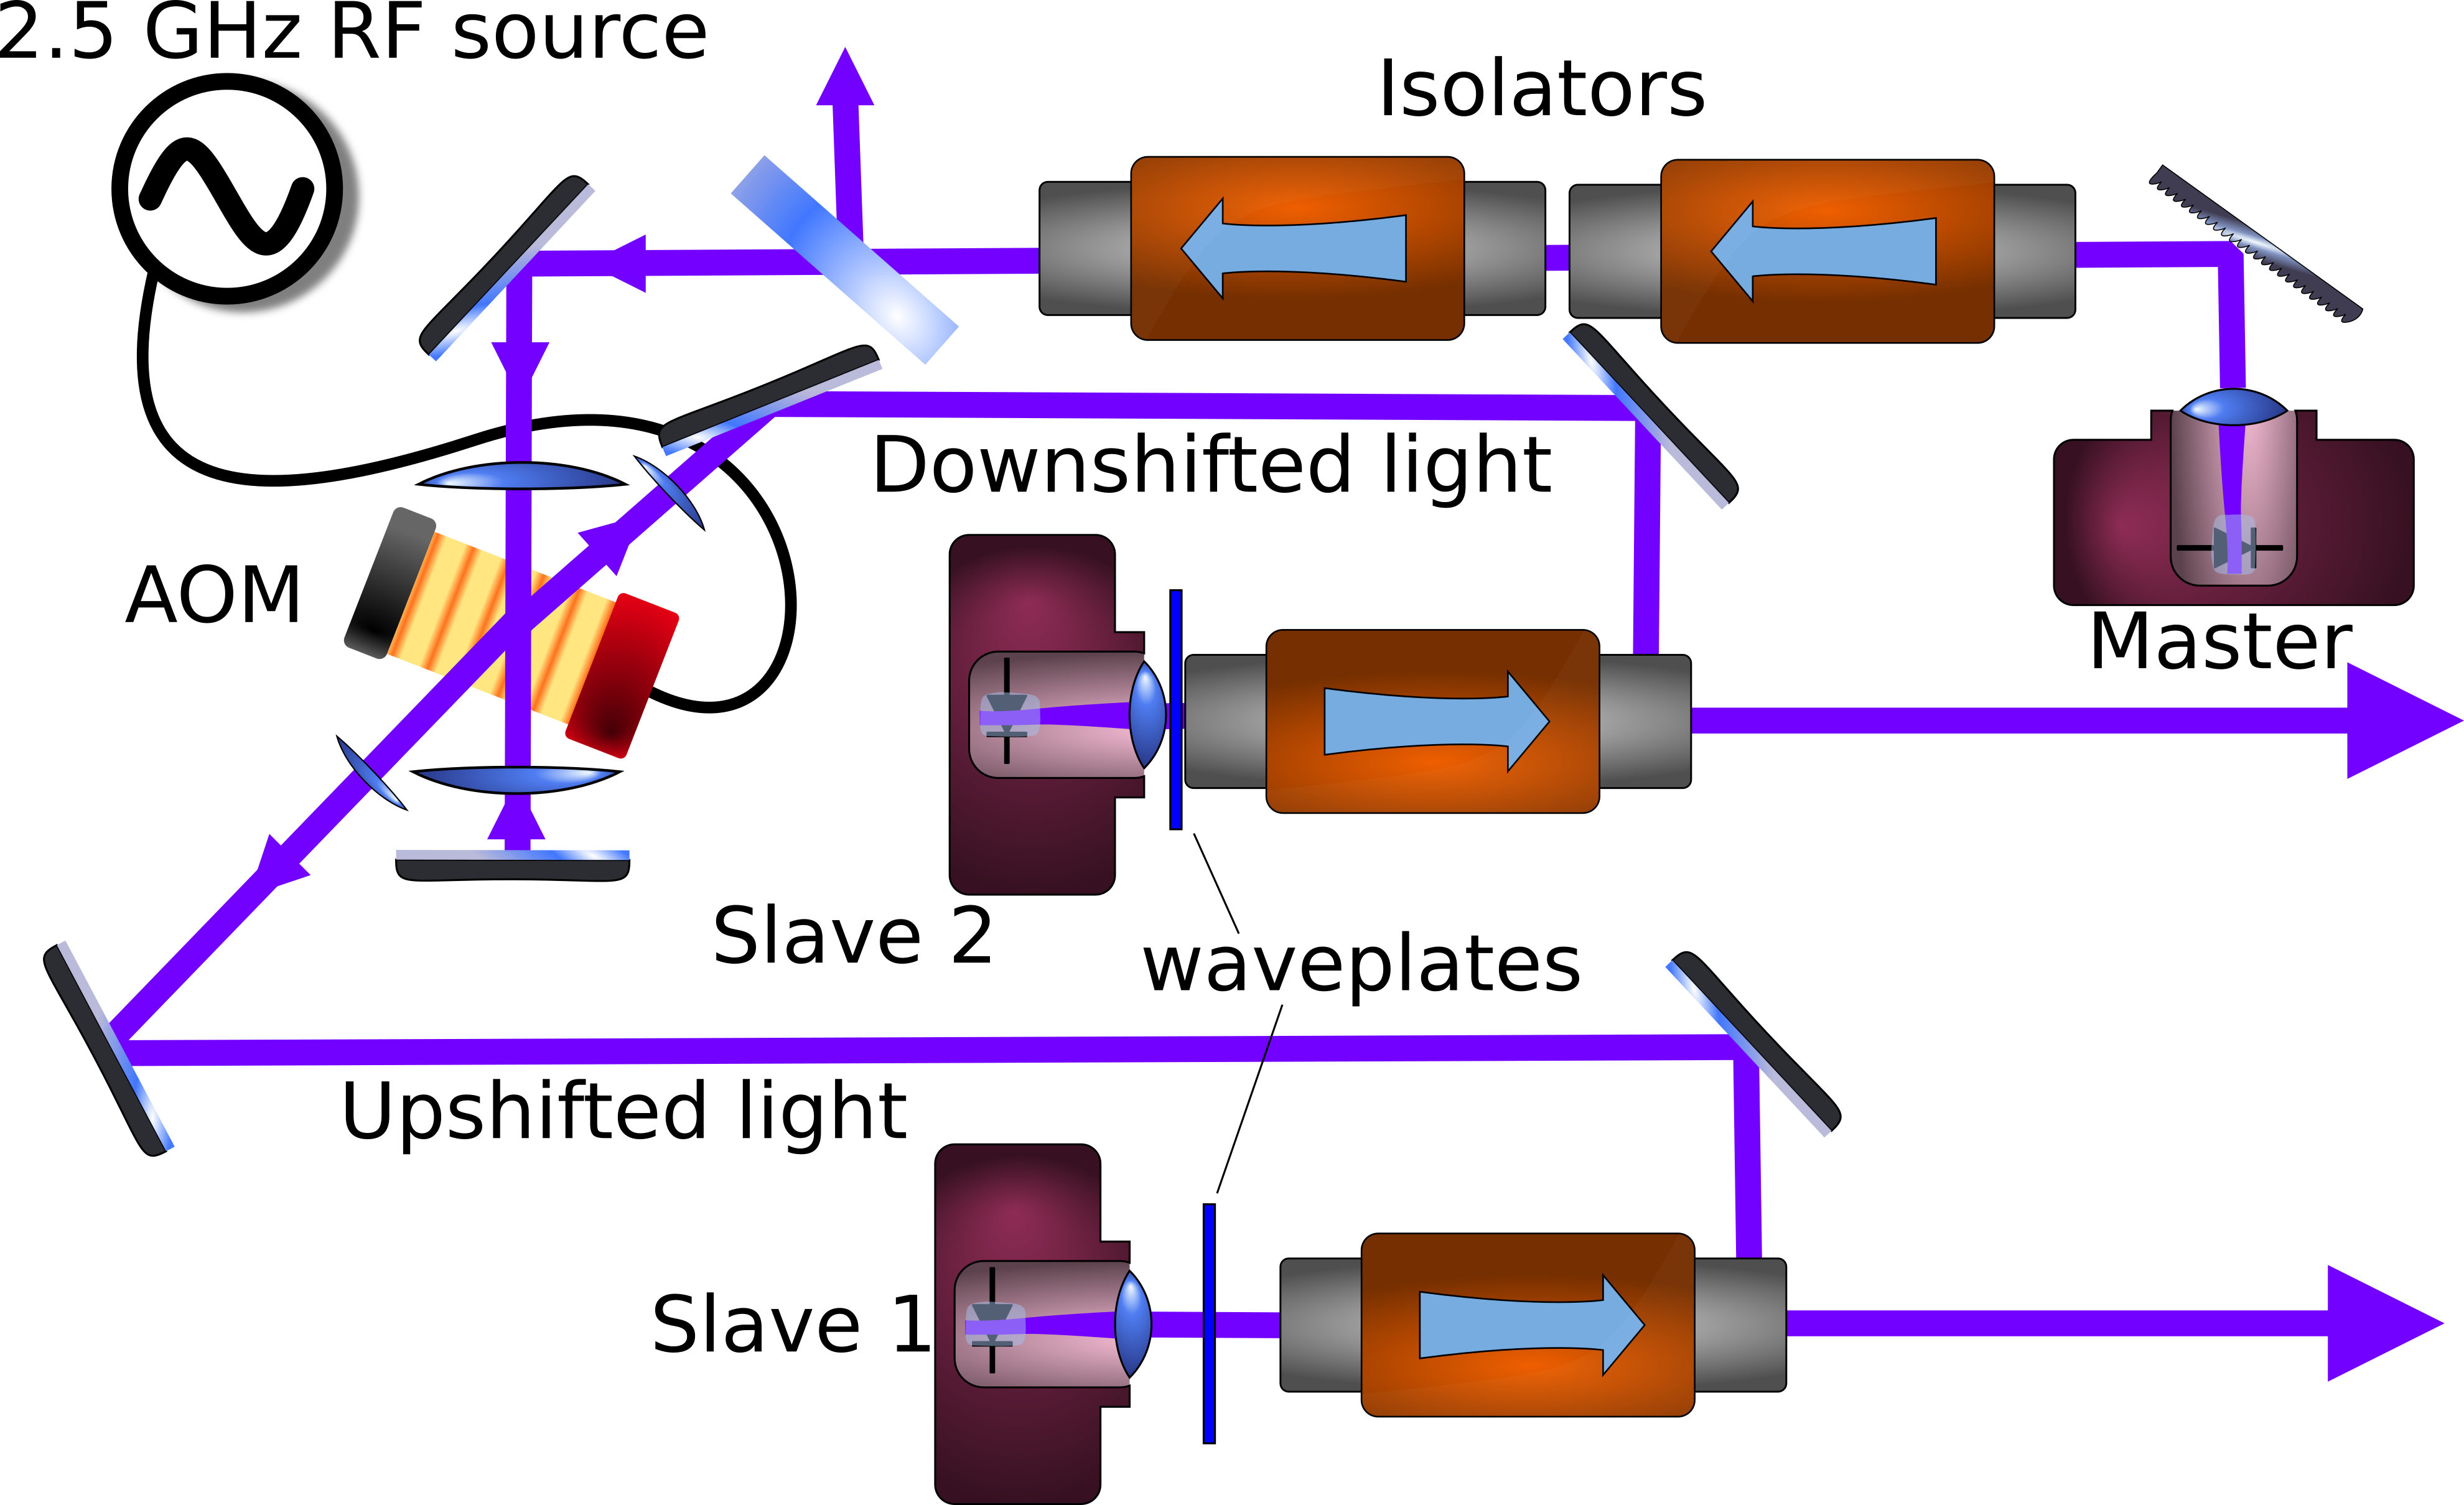
\includegraphics[width=1\textwidth]{diagramOfSetup3}}
    \caption[Diagram of the Setup]{\label{figdiagramOfSetup}
	A cartoon diagram of the basic pieces of the apparatus. The master laser is depicted on the upper right. This is followed by two optical isolators in series. After this, the AOM is depicted with the two beams coming out at exagerrated labels. These are then coupled into the exit ports of two other optical isolators. Finally, the final two beams come out the other end. Not pictured is the two waveplate setup that comes near the beam splitter. Also possibly not pictured are some half waveplates that go near the slave laser. 
    }
\end{figure}


There are three separate laser diodes in housings. One of them is designated the ``Master'' laser. The other two are designated ``Slave 1'' and ``Slave 2.'' 

The actual light used in the experiment comes out of the two slaves. The master laser is supposed to serve as a stable frequency reference so that the slave lasers can be seeded by it. Thus, the basic objective is to make a stable master laser tuned near the mean of the frequencies that we desire out of the slave lasers. This will then be shifted by an AOM and coupled into the slave lasers. The slave lasers are adjusted so that they are able to amplify the light from the AOM and lase with the same frequency as the light that comes out at the AOM. This is what is meant by "injection locking."

The advantage of this setup is that if the master laser were to drift, both slaves would presumably drift with it. As we will later see, the experiment is less sensitive to common mode drift between the two slave lasers than it is to the drifting of individual slaves.

The master laser is grating stabilized using an extended cavity formed by a  %look this up
lines/mm diffraction grating mounted on a piezoelectric mount. 

The master laser passes through two optical isolators. It is then passed through a pair of waveplates and a polarizing beam cube, which serves the dual purpose of allowing us to attenuate the portion of the beam that goes through the AOM and splitting off a beam that can be used in our spectrum analyzer. 

After this, the laser is passed twice through an Acousto-optic Modulator (AOM). It first passes through in one direction before being retroreflected and sent in the other direction. This splits off two beams, one of which is shifted upwards by 2.5 GHz and the other of which is shifted downward by 2.5 GHz. These two beams are then coupled through optical isolators into the two slave lasers. The outputs of these two lasers are what we use in our experiment to achieve stimulated Raman transitions. 

Both slaves are also redirected to the spectrum analyzer. 
